\documentclass{beamer}
\beamertemplatenavigationsymbolsempty
\usecolortheme{beaver}
\setbeamertemplate{blocks}[rounded=true, shadow=true]

% Красивый футер с номером кадра / общим числом
\setbeamertemplate{plain footline}{}
\setbeamertemplate{footline}[frame number]    % ← без {}
\setbeamertemplate{blocks}[rounded=true, shadow=true]
\setbeamertemplate{caption}[numbered]
\setbeamertemplate{caption label separator}{.\ }

%\usetheme{moloch}% modern fork of the metropolis theme


\usepackage[utf8]{inputenc}
\usepackage{amsmath,amssymb}
\usepackage{hyperref}

%%%%%%%%%%%

\usepackage{csquotes}
% === компактный стиль литературы ===
\usepackage[
  backend=biber,
  style=numeric-comp,   % числовой стиль → одна строка
  sorting=none,         % порядок как в .bib
  maxbibnames=3,        % «И др.» вместо всех авторов
  giveninits=true       % инициалы вместо имён
]{biblatex}

\addbibresource{sample.bib}

% убираем URL/DOI/издателя – меньше строк
\AtEveryBibitem{%
  \clearfield{url}
  \clearfield{doi}
  \clearfield{urldate}
  \clearlist{publisher}
}

\usepackage{array}
\usepackage{changepage}
\usepackage{caption}
\usepackage[T2A]{fontenc}
\usepackage[russian]{babel}


\usepackage{amsthm}

% Title Page Information
\title{Оптимизация архитектуры нейросети с контролем эксплуатационных характеристик на целевом устройстве}
\author{Фирсов Сергей \\ \vspace{5pt} Научный руководитель: к.ф.-м.н. О.Ю. Бахтеев}
\institute{Московский физико-технический институт}
\date{2025}

\begin{document}

\begin{frame}[plain]
    \titlepage
\end{frame} % 10 сек

%%%%%%%%%%%%%%%%%%%%%%%%%%%%%%%%%%%%%%%%%%%%%%%%%%%%

\begin{frame}{Цель исследования}

\begin{itemize}

    \item \textbf{Neural Architecture Search:} 
    Задача автоматизированного поиска оптимальной архитектуры нейросети. 

    \vspace{10pt}
    
    \item \textbf{Цель:} 
    Получать архитектуры решающие поставленную ML задачу, при этом удовлетворяя вычислительным или ресурсным ограничениям.
    
    \vspace{10pt}

    
    \item \textbf{Проблемы:} % Challenges Проблемы //// 
    \begin{itemize}
        \footnotesize
        \item {Обширное пространство для поиска}
        \item {Баланс точности и сложности}
        \item {Получение семейства решений}
    \end{itemize}
    \end{itemize}
 
\end{frame}

%%%%%%%%%%%%%%%%%%%%%%%%%%%%%
\begin{frame}{Постановка задачи} % == предлагаемый метод
\begin{itemize}

    \item Многоклассовая классификация. Выборка $
    \mathfrak D = \{(\boldsymbol{x}_i, y_i)\}_{i=1}^{\mathcal N},
    \ \boldsymbol{x_i} \in \mathbf X,\; y_i \in \mathbf Y. $

    \vspace{10pt}
    
    \item Модель --- нейронная сеть из повторяющихся блоков, каждый из которых представляется в виде DAG\footnote{\citeauthor{liu2019darts}, \citeyear{liu2019darts}: \citetitle{liu2019darts}}. Задача выбирать рёбра-операции $\boldsymbol{o}^{(m)}$ для каждой пары вершин в блоке. 
    
    \vspace{10pt}
    
    \item Для релаксации дискретной задачи выбора архитектуры в непрерывную, вводится \textit{смешанная операция}
    
    $$\hspace{-20pt}
    \widehat{\boldsymbol{g}}^{(i,j)}(\boldsymbol x) 
    \;=\; 
    \sum_{m=1}^k 
    \gamma^{(i,j)}_m \,\boldsymbol{o}^{(m)}(\boldsymbol x),
\ \ 
    \boldsymbol{\gamma}^{(i,j)}  \sim\; 
    \mathrm{GumbelSoftmax}\bigl(\boldsymbol{\alpha}^{(i,j)},\,t\bigr).
$$
\end{itemize}


    
\end{frame}


%%%%%%%%%%%%%%%%%%%%%%%%%%%%%%%%%%%%%%%%%%%%%%%%%%%%

\begin{frame}{Регуляризация сложности}


Вводится \textit{векторный параметр сложности}\footnote{\citeauthor{yakovlev2021neural}, \citeyear{yakovlev2021neural}: \citetitle{yakovlev2021neural}} $\boldsymbol{s}$, компоненты которого --- коэффициенты регуляризации по соответствующим операциям.
$$\boldsymbol{s} \in \Delta^{k-1}, \quad
\Delta^{k-1} \;=\; \bigl\{\,\boldsymbol{s}\in \boldsymbol R^k\mid \sum_{m=1}^k s_m = 1,\; s_m\ge0 \bigr\},$$
где $k = |\mathcal O|$,  $ \Delta^{k-1}$ \textit{симплекс} размерности $k-1$.

\vspace{10pt}

Определим функцию затрат Cost архитектуры $\gamma$ на основе $\boldsymbol{s}$:
$$Cost\bigl(\gamma;\,\boldsymbol{s}\bigr)
    \;=\; 
    \sum_{(i,j)\in E} \sum_{m=1}^k 
    \gamma^{(i,j)}_m \;s_m.$$

%Чем больше $s_m$, тем менее невыгодно использовать примитивную операцию $o_m$.
\end{frame}

%%%%%%%%%%%%%%%%%%%%%%%%%%%%%%%%%%%%%%%%%%%%%%%%%%%%

\begin{frame}{Теорема} % [plain,noframenumbering]
\small
% \textit{Стохастическое порождение $\gamma\sim GS$ вносит высокую дисперсию градиентов, особенно при малой температуре $t$. Так как математическое ожидание GS-вектора совпадает с обычным Softmax $\hat\gamma = \mathbb E[\gamma] = Softmax(\alpha/t)$, можно безопасно подменить $\gamma$ на $\hat\gamma$ в Cost части функции потерь, где важна стабильность. Формальную корректность такой подмены устанавливает следующая теорема.}

\begin{theorem}[Фирсов, 2025]
Пусть для каждого набора весов $\boldsymbol w\in\mathbb R^n$
и любого входа $\boldsymbol x\in\mathcal X$ функция
$$f(\boldsymbol\gamma)
   \;=\;
   \mathcal L_{\mathrm{task}}\!\bigl(\boldsymbol w,\boldsymbol\gamma\bigr)
    \ + \ \  \kappa\,\langle\boldsymbol\gamma,\boldsymbol s\rangle,
    \ \ \ \ \ \ \boldsymbol s\in\Delta^{k-1},$$
непрерывна и ограничена на симплексе
$\Delta^{k-1}
  =\bigl\{\boldsymbol\gamma\in\mathbb R^{k}\mid\sum_{i=1}^{k}\gamma_i=1,\;
          \gamma_i\ge 0\bigr\}$.
Положим
$$\boldsymbol\gamma(t)\sim\mathrm{GumbelSoftmax}(\boldsymbol\alpha,t),
   \qquad
   \boldsymbol{\bar\gamma}(t)=\mathrm{Softmax}\!\bigl(\boldsymbol\alpha/t\bigr)
               =\mathbb E\bigl[\boldsymbol\gamma(t)\bigr].$$
Тогда
$$\lim_{t\to 0^{+}}
       \mathbb E\bigl[f\bigl(\boldsymbol\gamma(t)\bigr)\bigr]
   \ \ \ = \ \ \ 
   f\!\bigl(\,\boldsymbol{\bar\gamma}(0)\bigr).$$
\end{theorem}

\end{frame}

%%%%%%%%%%%%%%%%
\begin{frame}{Оптимизационная задача}

Для генерации архитектуры вводится гиперсеть
$u_{\boldsymbol a}\colon \Delta^{k-1} \;\rightarrow\; \Gamma$  с параметрами $\boldsymbol a$, которая по заданному вектору сложности $\boldsymbol{s}\in\Delta^{k-1}$ порождает логиты
$\boldsymbol{\alpha}$, тем самым определяя архитектуру модели с учётом эксплуатационных характеристик.

\vspace{20pt}
% \begin{theorem}[Фирсов, 2025] \label{th:gs_softmax}
% \vspace{-20pt}
% $$\boldsymbol\gamma(t)\sim\mathrm{GumbelSoftmax}(\boldsymbol\alpha,t),
%    \ \ \ 
%    \boldsymbol{\bar\gamma}(t)=\mathrm{Softmax}\!\bigl(\boldsymbol\alpha/t\bigr)
%                =\mathbb E\bigl[\boldsymbol\gamma(t)\bigr].$$
% Тогда
% $$\lim_{t\to 0^{+}}
%        \mathbb E\bigl[f\bigl(\boldsymbol\gamma(t)\bigr)\bigr]
%    \ \ \ = \ \ \ 
%    f\!\bigl(\,\boldsymbol{\bar\gamma}(0)\bigr).$$
% \end{theorem}

%\rule[0pt]{310pt}{0.5pt} %\linewidth
\vspace{20pt}
Оптимизационная задача:
$$ \hspace{-5pt}\boxed{\mathbb E_{\boldsymbol s\sim U(\Delta^{k-1})} \ \Bigl[ \ {\mathbb E_{\boldsymbol\gamma\sim\mathrm{GS}(\boldsymbol\alpha(\boldsymbol s),t)} \mathcal L_{\text{task}}(\boldsymbol w,\boldsymbol\gamma)} \ +\  \kappa\,Cost\bigl(\boldsymbol{\bar\gamma}(\boldsymbol s);\boldsymbol s\bigr) \ \Bigr] \rightarrow \min_{\boldsymbol w,\boldsymbol a}}  
$$


\end{frame}

%%%%%%%%%%%%%%%%%%%%%%%%%%%%%%%%%%%%%%%%%%%%%%%%%%%%

\begin{frame}{Иллюстрация}

\begin{figure}
        \centering
        \includegraphics[width=1\linewidth]{Idea.png}
        Иллюстрация предлагаемого метода.
       
\end{figure}

\begin{itemize}
    \item Предлагается использовать векторный параметр сложности $\boldsymbol{s}$, компоненты которого --- коэффициенты регуляризации по соответствующим операциям.
    \item Гиперсеть на основе $\boldsymbol{s}$ генерирует архитектурные параметры для нейросети.
\end{itemize}

\end{frame}


%%%%%%%%%%%%%%%%%%%%%%%%%%%%%%%%%%%%%%%%%%%%%%%%%%%%

\begin{frame}{Постановка эксперимента}
\begin{itemize}
    \item Эксперименты поставлены для подтверждения работоспособности метода и иллюстрации его возможностей.
    \vspace{10pt}
    \item Представленный эксперимент проводится на выборке Fashion-MNIST.
    \vspace{10pt}
    \item Рассматриваются модели из 3 блоков по 4 вершины. Доступные операции \(3{\times}3\) convolution, \(3{\times}3\) max-pooling и identity (передача данных без изменений).
    \vspace{10pt}
    \item Параметры $\boldsymbol w$ и параметры гиперсети $\boldsymbol a$ тренировались с помощью оптимизаторов Adam. 
    \vspace{10pt}
    \item Температура Gumbel–Softmax линейно уменьшалась от \(t{=}1.0\) до \(t{=}0.2\) по эпохам. 

\end{itemize}
\end{frame}

%%%%%%%%%%%%%%%%%%%%%%%%%%%%%%%%%%%%%%%%%%%%%%%%%%%%
\begin{frame}{Получение моделей}
Получено \textbf{семейство} нейронных сетей, из которого для анализа выделяется четыре архитектуры, соответствующие приведённым ниже векторам сложности $\boldsymbol{s} = (pool, ident, conv)$. Компоненты вектора являются штрафами за соответствующие операции.
\[
\text{(A) } (0.33,0.33,0.33),\quad
\text{(B) } (0.15,0.15,0.70),
\]
\[
\text{(C) } (0.70,0.15,0.15),\quad
\text{(D) } (0.15,0.70,0.15).
\]
Представленные архитектуры отражают равномерный штраф за операции (А), увеличенный за свёртки (B), увеличенный за пулинг (C) и увеличенный за пропуск (D). 


\end{frame}

\begin{frame}{Распределение операций}

\begin{figure}[!ht]
    \centering
    % --- 1-я строка ---
    \begin{minipage}[t]{0.48\linewidth}
        \centering
        \includegraphics[width=\linewidth]{Figure_1_no_penalty.png}\\
        (A) равномерный штраф
    \end{minipage}\hfill
    \begin{minipage}[t]{0.48\linewidth}
        \centering
        \includegraphics[width=\linewidth]{Figure_1_conv_penalty.png}\\
        (B) увеличенный за свёртки
    \end{minipage}

             
    \label{fig2}
\end{figure}
    Статистика по операциям для архитектур эксперимента 1.
\end{frame}

\begin{frame}{Распределение операций}

\begin{figure}[!ht]
    \centering
    % --- 2-я строка ---
    \begin{minipage}[t]{0.48\linewidth}
        \centering
        \includegraphics[width=\linewidth]{Figure_1_pool_penalty.png}\\
        (C) увеличенный за пулинг
    \end{minipage}\hfill
    \begin{minipage}[t]{0.48\linewidth}
        \centering
        \includegraphics[width=\linewidth]{Figure_1_ident_penalty.png}\\
        (D) увеличенный за пропуск
    \end{minipage}

    
    \label{fig3}
\end{figure}
 Статистика по операциям для архитектур эксперимента 1.   
\end{frame}
%%%%%%%%%%%%%%%%%%%%%%%%%%
\begin{frame}[t]{Результаты}

  
  \begin{table}[h!]
    \centering
    \small
   % \begin{tabular}{|c|c|c|c|}
   
   \begin{tabular}{b{4.5cm}|b{1.2cm}|m{1.2cm}|m{1.2cm}|m{1.2cm}||}
   \hline
     \textbf{Модели} & \textbf{A} & \textbf{B} & \textbf{C} & \textbf{D} \\
    \hline
    \hline
    \textbf{Accuracy} &  82.5\% & 79.2\% &  \textbf{85.0\%} & 81.4\\
    \hline
    \textbf{Количество параметров} & 38\,304 & \textbf{5\,120} & \textbf{143\,488} &12\,320 \\
    \hline
    \textbf{Количество pooling} & 12 & 17 & \textbf{0} &18\\
    \hline
    \textbf{Количество convolution} & 6 & \textbf{0} & 13& 9 \\
    \hline
    \textbf{Количество identity} & 10 & 11 & 15 & \textbf{1} \\
    \hline
    \end{tabular}
     Сравнение параметров полученных архитектур. \textbf{(A)} равномерный штраф, 
             \textbf{(B)} увеличенный за свёртки, 
             \textbf{(C)} увеличенный за пулинг, 
             \textbf{(D)} увеличенный за пропуск.
  \end{table}

    Результаты подтверждают корректность работы предлагаемого метода. При увеличении штрафа за операцию --- уменьшается её использование в модели. Регуляризация позволяет учитывать различные эксплуатационные ограничения без необходимости дообучения модели на них.
\end{frame}

%%%%%%%%%%%%%%%%%%%%%%%%%%%%%%%%%%%%%%%%%%%%%%%%%%%%

\begin{frame}{Выносится на защиту}
\begin{itemize}
    \item Предложен метод позволяющий получать семейство моделей с возможностью контроля сложности обучения и аппаратных ограничения.
    \item Метод обладает возможностью получать архитектуры моделей за счёт изменения вектора параметра сложности без необходимости дополнительного дообучения.
    \item Вычислительные эксперименты подтверждают работоспособность метода и демонстрируют заявленную гибкость получаемого решения.
\end{itemize}

\vspace{10pt}
Результаты работы доложены на конференции МФТИ и в университете Сириус.

В рамках дальнейшего развития метода планируется добавление многокритериального учета сложности и проведение полноформатного сопоставления результатов с классическими NAS-подходами.

\end{frame}

%%%%%%%%%%%%%%%%%%%%%%%%%%%%%%%%%%%%%%%%%%%%%%%%%%%%


\begin{frame}[plain,noframenumbering, t]{Список литературы}
  \tiny
  \nocite{*}                 % напечатать ВСЁ из .bib
  \printbibliography
\end{frame}

%%%%%%%%%%%%%%%%%%%%%%%%%%%%%%%%%%%%%%%%%%%%%%%%%%%%

\begin{frame}[plain,noframenumbering]{Примечание. Клетка}
    \begin{figure}
        \centering
        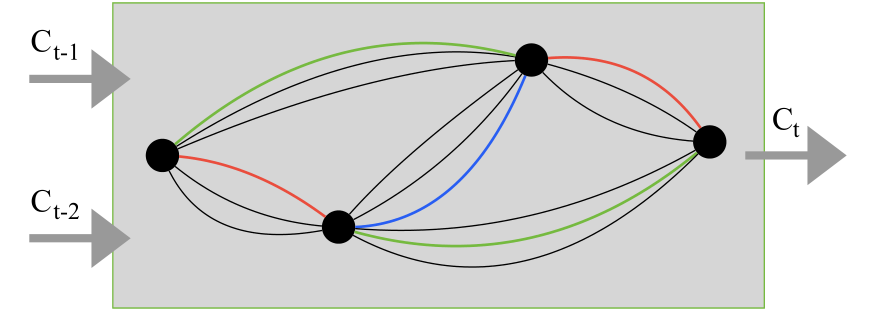
\includegraphics[width=\linewidth]{Cells_DARTS_1_1.png}
        Иллюстрация клетки.
       
    \end{figure}
\end{frame}
\begin{frame}[plain,noframenumbering]{Примечание. Гиперсеть}
     Введём \textit{гиперсеть} $\boldsymbol{u}_{\boldsymbol a}$ с параметрами $\boldsymbol a$, которая на основе $\boldsymbol{s}$ строит логиты $\boldsymbol\alpha^{(i,j)}$ для каждого ребра $(i,j)$ как взвешенную комбинацию заранее выученных логитов опорных архитектур $\boldsymbol\alpha_{\text{ref},r}^{(i,j)}$, полученных в процессе оптимизации гиперсети. По вектору сложности $\boldsymbol{s}$ вычисляются веса интерполяции

$$
  w_r(\boldsymbol{s})
  =  
  \frac{\exp\bigl(-\|\boldsymbol{s} - \boldsymbol{s}_{\text{ref},r}\|^2\bigr)}
       {\displaystyle\sum_{l=1}^{m}\exp\bigl(-\|\boldsymbol{s} - \boldsymbol{s}_{\text{ref},l}\|^2\bigr)},
  \quad
  r = 1,\dots,m,
$$

где $\boldsymbol{s}_{\text{ref},r}\in\Delta^{k-1}$ — $r$-я опорная точка, а $m$ — их общее число. Затем итоговые логиты для ребра $(i,j)$ вычисляются как

$$
  \boldsymbol\alpha^{(i,j)}(\boldsymbol{s})
  \;=\;
  \sum_{r=1}^{m} w_r(\boldsymbol{s})\;\boldsymbol\alpha_{\text{ref},r}^{(i,j)}.
$$
\end{frame}

\begin{frame}[plain,noframenumbering]{Примечание. Оптимизационная задача}
    
$$
\mathbb E_{\boldsymbol s\sim U(\Delta^{k-1})} \ \Bigl[ \ {\mathbb E_{\boldsymbol\gamma\sim\mathrm{GS}(\boldsymbol\alpha(\boldsymbol s),t)} \mathcal L_{\text{task}}(\boldsymbol w,\boldsymbol\gamma)} \ +\  \kappa\,Cost\bigl(\boldsymbol{\bar\gamma}(\boldsymbol s);\boldsymbol s\bigr) \ \Bigr] \rightarrow \min_{\boldsymbol w,\boldsymbol a} \ , 
$$
где $\boldsymbol w$ --- все параметры внутри примитивных операций $\mathbf{o}^{(m)}$;
$\boldsymbol a$ --- параметры гиперсети $\boldsymbol{u}_{\boldsymbol a}$, которая генерирует логиты $\boldsymbol\alpha^{(i,j)}$ для всех $(i,j)\in E$ при подстановке $\boldsymbol{s}$;
$\boldsymbol{s} = (\boldsymbol{s}\_1,\dots,\boldsymbol{s}\_k)\in\Delta^{k-1}$ --- вектор сложности, порождённый из равномерного распределения на симплексе $\Delta$;
$\mathcal L_{\text{task}}$ --- кросс-энтропия по обучающей выборке;
$\boldsymbol\gamma^{(i,j)}(\boldsymbol{s})$ --- веса операций на ребре $(i,j)$, получаемые через Gumbel‐Softmax от логитов $\boldsymbol{u}_{\boldsymbol a}^{(i,j)}(\boldsymbol{s})$; 
$\boldsymbol\gamma$ --- вектор состоящий из $\boldsymbol\gamma^{(i,j)}$;
$\boldsymbol{\bar\gamma} = \mathbb E[\boldsymbol{\gamma}(t)]$; 
$Cost$ --- штраф за использование дорогих операций;
$\kappa$ --- гиперпараметр, управляющий важностью штрафа.

\end{frame}
\end{document}

